\pdfminorversion=4
\documentclass[notes=hide]{beamer}
%\includeonlyframes{results}
\usepackage[overlay,absolute]{textpos}
\usepackage{natbib}
\usepackage{tikz}
\tikzstyle{every picture}+=[remember picture]
\tikzstyle{na} = [baseline=-.5ex]
\setlength{\TPHorizModule}{\paperwidth}
\setlength{\TPVertModule}{\paperheight}
\definecolor{UniGray}{RGB}{94, 94, 87}
\definecolor{UniRed}{RGB}{90, 0, 20}
\setbeamercolor{alert}{fg=red}
\setbeamercolor{block title}{bg=white}
\setbeamercolor{block body}{bg=white}
\newcommand{\mpoint}[1]{
  {\usebeamercolor[fg]{alert}#1}
}
\setbeamerfont{small}{size=\scriptsize}
{
\mode<presentation>
{
  \usetheme[footheight=0.3cm]{boxes}
  \addfootboxtemplate{\color{UniGray}}{\hspace{0.0cm}
    \color{white}
    
\includegraphics[height=0.8cm]{IUP-Logo.pdf}
    \hspace{2cm}
    Mathias Palm 
    \hfill
    \hspace{2cm}
%    \includegraphics[height=0.8cm]{RAM-Logo.eps}
%    \hfill\color{white}\insertshorttitle\hfill
%    \insertshortauthor
    \insertframenumber / \inserttotalframenumber
    \hfill
  } 
  % or ...

  \setbeamercovered{transparent=0}
}

\beamertemplatenavigationsymbolsempty

\usepackage[english]{babel}
\usepackage[latin1]{inputenc}
\usepackage{graphicx, colortbl}
\usepackage{times}
\usepackage[T1]{fontenc}



\title {SFIT4 -- Retrieval parameters}

\author[Mathias Palm]{Mathias Palm} 
\institute[] {Institute of Environmental Physics\\
  Universit�t Bremen\\Germany}


\date{Boulder, 2019}

\begin{document}

\begin{frame}
\maketitle
\end{frame}

\begin{frame}
  \Huge{Retrieval parameters}
\end{frame}

\begin{frame}
  \begin{textblock*}{\textwidth}(0.1\textwidth,0.2\textheight)
    \includegraphics<2>[width=\textwidth]{output_sfit4_retrieval.png}
  \end{textblock*}
  \frametitle{Retrieval parameters}
  \framesubtitle{Overview}
  \begin{description}[\hspace{0.5cm}]
  \item[rt]   The main parameter rt can be used to switch off and one the retrieval altogether.
  \item[rt.lm] Switches on or off the Levenberg-Marquardt iteration scheme.
  \item[rt.convergence] the iteration is considered converged when
    rt.convergence > D\_CHI = (CHI\_2\_MAX$_{i-1}$ - CHI\_2\_MAX$_i$) 
  \item[rt.max\_iteration] maximum number of iterations  
  \end{description}
  \only<3->{For all retrieval parameters a apriori is given and a standard deviation sigma in the form}
  \begin{description}[\hspace{0.5cm}]
  \item[rt.x.apriori] <3>the apriori of a given value. It is actually
    applied in the forward calculation. Meaning it can also be used in forward calculations.
  \item[rt.x.sigma] <3>the entry in the $S_A$ matrix corresponding to this parameter.
  \end{description}
\end{frame}

\begin{frame}
  \frametitle{Retrieval parameters}
  \framesubtitle{Wave number scaling and shifting}
  \begin{description}[\hspace{0.5cm}]
  \item[rt.wshift] wave number shift.
    \begin{itemize}
    \item Shift works on the internal grid {\bf band.X.calc\_point\_space}
    \item This is only useful for
      microwindows (small) because the mismatch is a wavenumber
      dependent polynomial. For small wave number regions, this can be
      approximated by a shift.
    \item This is on top of rt.wave\_factor, which is a scaling.
    \item The artificial grid needs to be more dense than the measured grid
    \end{itemize}
  \item [rt.dwshift] wave number shift for each retrieved gas
    separately, except the first retrieved one.
    \begin{itemize}
    \item all lines of each gas are shifted by the same amount (!!!)
    \end{itemize}
  \end{description}
\end{frame}

\begin{frame}
  \begin{textblock*}{\textwidth}(0.1\textwidth,0.1\textheight)
    \includegraphics<2>[width=\textwidth]{zshift_wrong.png}
  \end{textblock*}
  \frametitle{offset in window}
  \begin{description}[\hspace{0pt}]
  \item[band.zshift] calculates and retrieves an offset in the microwindow. Two types:
    \begin{description}
    \item[.type = 1] retrieves the offset in this MW \alert<1>{ONLY ONE!!!}
    \item[.type = 2] <3->uses the offset which is retrieved in another microwindow. \alert<1>{THIS MUST BE LATER THAN THE MW USED FOR \bf{ZSHIFT.TYPE=1}} 
    \end{description}
    \item[band.zshift.apriori] <3->is also an {\bf FW parameter}
    \only<4->{\alert{RETRIEVAL ONLY POSSIBLE IF THERE IS AN SATURATED PART IN THE MW.} }
  \end{description}
\end{frame}
\begin{frame}
  \frametitle{channeling in window}
  \begin{textblock*}{0.8\textwidth}(0.1\textwidth,0.2\textheight)
    \includegraphics<2>[width=\textwidth]{Channeling.png}
  \end{textblock*}
  The channeling in a MW is calculated via
  \begin{description}
  \item[band.x.beam] = 1,2 The beams with the numbers 1 and 2 are caclulated
  \item[band.x.beam.model] = IP, PS which one is better has to be checked.
  \item[band.x.beam.1.apriori] = AMP, FREQ,PHAS,SLOPE defines the apriori values of the beam 1
  \item[band.x.beam.1.sigma] standard deviations for all parameters, i
  sigma = 0, parameter is not retrieved,
  \end{description}
\end{frame}

\begin{frame}
  \begin{textblock*}{0.8\textwidth}(0.1\textwidth,0.2\textheight)
    \includegraphics<2>[width=\textwidth]{Backgn.png}
  \end{textblock*}
  \frametitle{rt.slope and rt.background} rt.slope and rt.background
  can be used to model a sensitivity function of the instrument,
  caused by a filter or the wave number dependent sensitivity of the
  instrument itself.

  A function
  \begin{equation}
    \mbox{rt.slope}*\nu + \mbox{rt.background}*\nu^2 
  \end{equation}
  is multiplied to the calculated spectrum.  
\end{frame}

\begin{frame}
  \frametitle{Retrieval parameters}
  \framesubtitle{Construction of the $S_A$ matrix.}
  The $S_A$ matrix is constructed from the
  sigma values given. How this is actually done, depends on the
  parameters. In principle the $S_A$ is constructed as a diagonal
  matrix and inverted in the code to yield the $S_A^{-1}$ matrix. Some
  caveats:
  \begin{overlayarea}{\textwidth}{0.7\textheight}
    \only<1>{
  \begin{description}[\hspace{.5cm}]
  \item[gas.profile.x.correlation] off diagonals using the sigma
    values as maxima
    \begin{description}[\hspace{.5cm}]
    \item[.type = 1] gaussian with FWHM = .width
    \item[.type = 2] exponentially with FWHM = .width
    \item[.type = 3] not used
    \item[.type = 4] the $S_A$ matrix is read in from file.sa\_matrix
    \item[.type = 5] the $S_A^{-1}$ matrix is read in from file.sa\_matrix
    \end{description}
  \end{description}
  }
  \only<2>{
  \begin{description}[\hspace{.5cm}]
  \item[gas.profile.x.regmethod] lets you chose between OE
    optimization and the Thikonov-Phillips regularization with L1
    constraint (smoothness constraint)
    \begin{description}[\hspace{.5cm}]
    \item[.type = 'OE'] optimal estimation (Rodgers, 2000)  
    \item[.type = 'TP'] Thikonov-Phillips with smoothness constraint
      \begin{description}[\hspace{.5cm}]
      \item[.lambda] strength of the regularization in TP. The higher the value the less is the regularization.
      \end{description}
      The smoothness constraint is calculated from file.stalayers in
      order to adapt for non-unique altitude layering. The matrix is
      scaled using the gas.profile.x.sigma values.
    \end{description}
  \end{description}
  }
  \end{overlayarea}
\end{frame}


\begin{frame}
  \begin{textblock*}{\textwidth}(0.0\textwidth,0.59\textheight)%
    \only<3>{\tikz \draw[red,very thick] (0,0) ellipse (4cm and 0.5cm);}
  \end{textblock*}
  \frametitle{Retrieval parameters}
  \framesubtitle{SFIT4 retrieval diagnostics}
  \vspace{-0.5cm}
  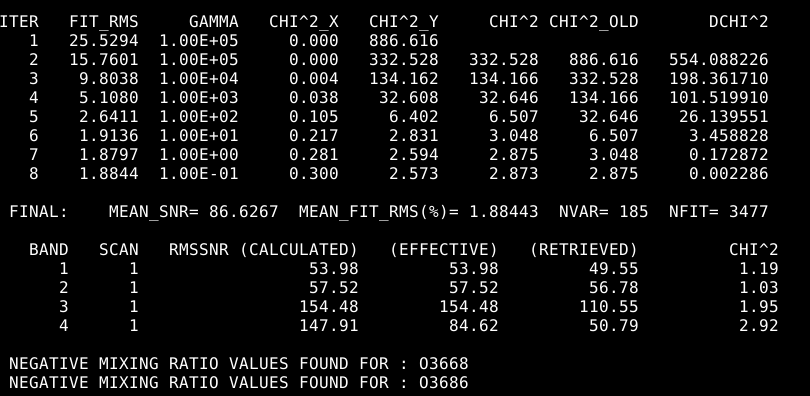
\includegraphics[width=\textwidth]{output_sfit4_retrieval.png}
  \begin{overprint}[\textwidth]
    \onslide<1>
    \begin{description}
    \item[FIT\_RMS] mean variance of the residuum
    \item[GAMMA] the Levenberg Marquardt Parameter
    \item[CHI\_2\_X] A measure of the deviation of the retrieved state from the A PRIORI
    \end{description}
    \onslide<2>
    \begin{description}
    \item[CHI\_2\_Y] A measure for the retrieval quality
    \end{description}
    \begin{equation*}
      \chi_Y^2 = \frac{(y_M - y_C)^T S_\epsilon (y_M - y_C)}{m}
    \end{equation*}
    $\chi_Y^2=1$ if the residuum is reduced to the noise as specified in $S_\epsilon$
    \onslide<3>
    \begin{itemize}
    \item     In the lower half, the retrieval diagnostics for the last calculation are shown for each MW.
    \item A warning if retrieved profiles have negative parts 
    \end{itemize}
    \onslide<4>
    Iteration stopped if either DCHI < rt.convergence or ITER > rt.max\_iteration, what ever comes first.
  \end{overprint}
\end{frame}

\begin{frame}
  \frametitle{The finish}
  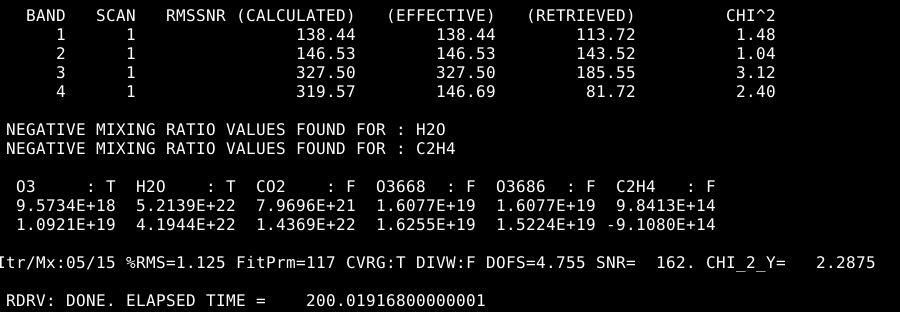
\includegraphics[width=\textwidth]{output_sfit4_finish.png}
  \end{frame}
\end{document}
 